\chapter{Development Process}


\section{Software Process}
% https://www.wikipendium.no/TDT4140_Programvareutvikling/nb/#kapittel-2-software-processes

% Incremental development etc. \#agile
% \large{Where everything I learned in PU should shine!}

Even though I have developed the Nevrolens application by myself, I have strived to use best practices for a software development workflow. These practices have generally grown out of the the needs of a multi-developer setting, enabling simpler use of collaboration and version control. Though their value possibly increases exponentially by the number of team members, I have found value in the structure and clarity I find in the workflow. 

\begin{figure}[h]
    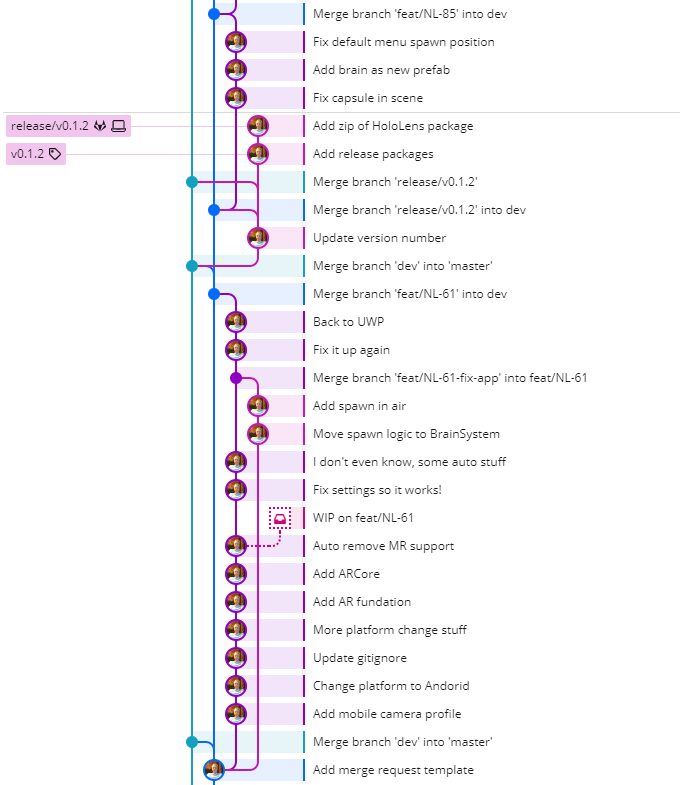
\includegraphics[width=0.33\textwidth]{fig/gitkraken_gitlog}
    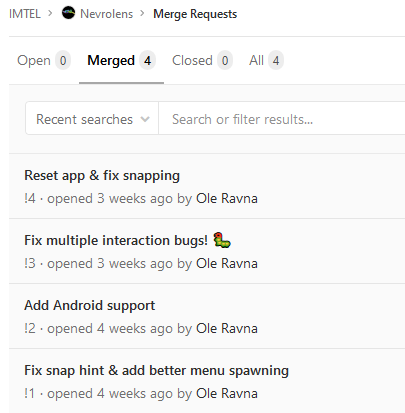
\includegraphics[width=0.33\textwidth]{fig/mergerequests}
    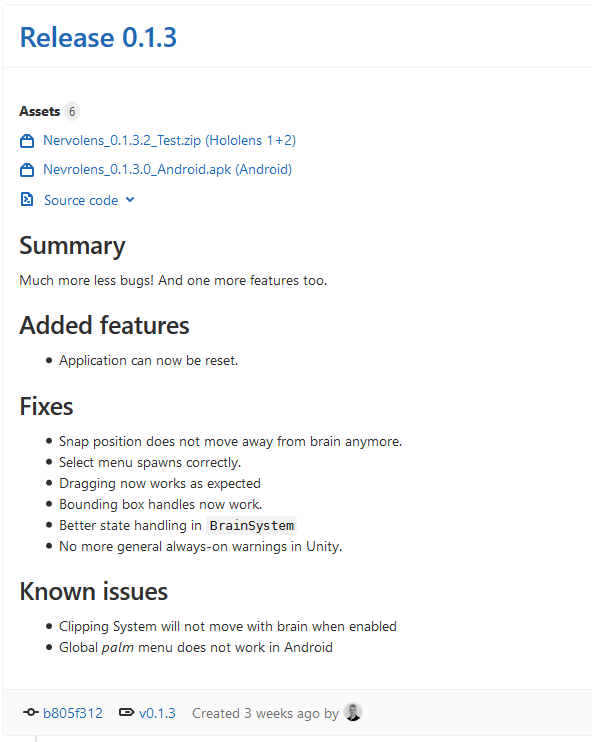
\includegraphics[width=0.33\textwidth]{fig/release_gitlab}
    \caption{Feature branches, merge requests and releases.}
\end{figure}

My workflow is based on \textit{Gitflow}, a workflow framework optimized for continuous software development. In short, this is just a very basic rule set for branch-naming and the sanctity of the master-branch (requiring merge requests of only product ready code), within the version control system \nameref{chap:git}. It does however act as a fundament which enables practices like rapid release cycles, because of the clearly define production ready state, and the integration with lean development technics like Kanban. This stems from the parallels between feature-branches in Gitflow and the \textit{ticket} in Kanban. In practice, this means that tickets, with issues or new features for the app, are created on in the \textit{Backlog} column of the Kanban board and are then moved to \textit{Doing} column simultaneously as a feature-branch is created with the ID of the ticket, e.g. \texttt{feat/NL-42}. All of this is automated in the Git management tool \nameref{chap:gitkraken}, which manages both the git-repo and the Kanban board.

\begin{figure}[h]
    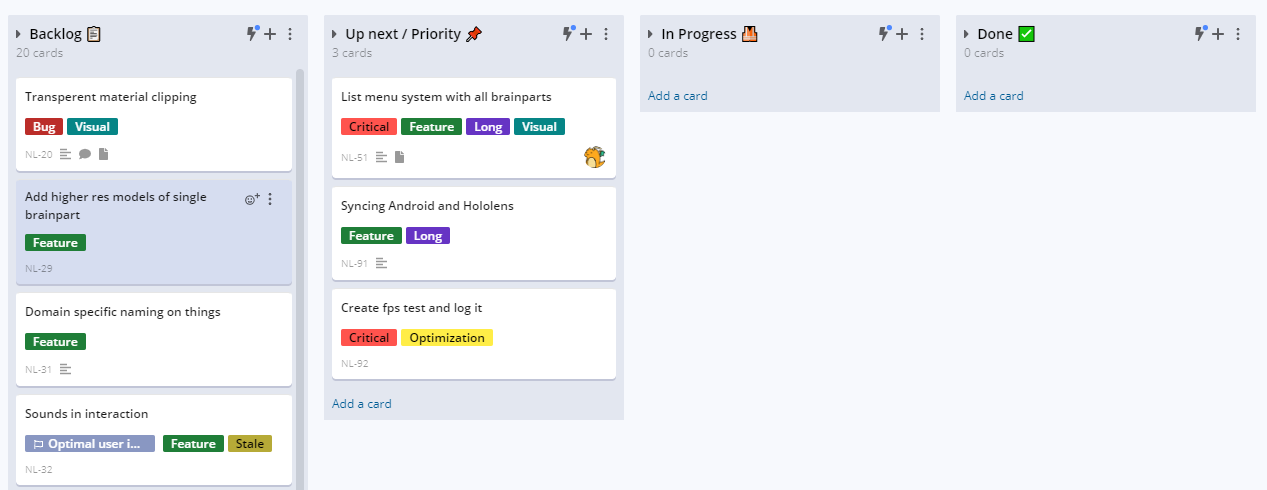
\includegraphics[width=\textwidth]{fig/kanban2}
    \caption{A snapshot of the Kanban board in GitKraken, after a development sprint, when completed tickets are archived (closed).\\ Note: \textit{Priority} acts as pined tickets on \textit{Backlog}, as the backlog tends to sizeable.}
    \label{fig:kanban}
\end{figure}

This workflow, by design, supports an agile development process. Agile approaches to software development are generally human-centered, valuing individuals and interactions over processes and tools\footnote{The Agile Manifesto https://agilemanifesto.org/}, and focused on iterating rather than upfront planning. This is ideas which are beneficial for single-developer or small teams especially when developing for new platforms like the HoloLens 2. 
While the project aims for an agile approach, the sprint cycle core to the agile development, where stakeholders are involved for regular feedback, has, due to a number of factors like COVID-19, only really been done for one cycle. However, the steps taken for an agile workflow should enable more agile development for the master project.

% One thing that I have not incorporated in to the workflow is user stories. The tickets in \autoref{fig:kanban} are written only for my understanding and will seem confusing and untidy for others. By using the concept of user stories 

% and will limited testing possibilities due to COVID-19 


% this enables me as a developer to test the product rapidly against users. 
% , this means having rules for branch naming, creating merge requests when merging to the `master`-branch, and 